\documentclass[12pt]{article}

\usepackage{amsmath}
\usepackage[margin = 1in]{geometry}
\usepackage{graphicx}
\usepackage{booktabs}
\usepackage[colorlinks=true, citecolor=blue]{hyperref}
\usepackage{underscore}

\title{Using Statistical Modeling to Estimate the Chances of Success of College Basketball Transfers}
\author{Miles Kee}

\begin{document}
\maketitle

\begin{abstract}
When the NCAA decided to eliminate the rule of athletes needing to sit out a season after transferring due to the COVID-19 pandemic, it created a frenzy in the college basketball world. Record numbers of players transferring were seen immediately after this ruling. Since then, the NCAA has decided to make this elimination permanent. This, combined with student athletes newfound ability to profit off their name, image, and likeness, has turned the college basketball offseason into a scene that is more akin to the free agency period in professional sports. Over 1500 players entered the transfer portal during the 2023 offseason. College coaches have began rebuilding their entire teams using the transfer portal instead of the traditional program-building methods of recruiting well and emphasizing development. New St. John's coach Rick Pitino was hired in March, and by early May, he had already brought in eight new transfers while losing another eight to the transfer portal. This type of roster turnover has become routine in the college game, especially when a coach is fired or hired. 
\end{abstract}

\section{Introduction}
The goal of this project is to use statistical modeling techniques to more efficientl


\section{Data}
\label{sec:data}
The data for this project comes courtesy of \href{barttorvik.com}{barttorvik.com}. The files titled "transferYEAR" contain each player who transferred schools in a given year. For example, the file named "transfer22" contains each transfer that started at their new school during the 2021-2022 season. The rows in each of the transfer files are as follows: player\_name, team, conf, min\_per, ORtg, usg, eFG, ORB\_per, DRB\_per, AST\_per, TO\_per, blk\_per, stl\_per, ftr, yr, ht, new.school, and dbpm. \autoref{tab:data-expl} explains what each of these variables means. eFG percentage was chosen instead of traditional FG percentage because it properly weighs the added impact of a three pointer when compared to a two pointer by multiplying three pointers made by 1.5. The formula is \(eFG=(2PM+1.5*3PM)/(FGA)\), where 2PM and 3PM are two and three pointers made, respectively, and FGA is field goals attempted. The offensive statistics in the data are ORtg, usg, eFG, ORB\_per, AST\_per, TO\_per, and ftr. The defensive statistics are DRB\_per, blk\_per, stl\_per, and dbpm. There are many more stats available to track a player's offensive impact when compared to the stats available to track a player's defensive impact. Defense is much more nuanced, as not every good defensive play shows up in a box score. This is why dbpm is used, as it reflects a team's full defensive performance when a player is on the court, allowing us to better quantify and inherently non-quantifiable concept. The data contains files titled "statsYEAR," which are used to look at a player's stats the year after he transferred. The same statistics are used for both the transfer and stats files. Finally, the "fulldata" file contains each transfer from 2021-2023, their stats from the year before they transferred, and their stats from the year after they transferred. The years 2021, 2022, and 2023 are looked at because these are the years the "free agency" aspect of the transfer portal started. The 2024 transfers are excluded from this study because at the time it was conducted, the new season had not given a significant enough sample size to evaluate the players' performances. This leaves us with 2093 players in the "full data" file. The target variables to predict are ORtg and dbpm, as those do the best job of encapsulating a player's impact on offense and defense, respectively, into a single number.
\subsection{Feature Engineering}
\label{subsec:feature-eng}
Once the data was loaded in, I added some features to the data. The variable created called "fromp5" indicates whether a player transferred from a power conference school which in this case are: Big East, Big 12, Big 10, Pac 12, ACC, and SEC. The variable created called "top5" indicates whether a player transferred to a power conference school. The variable called "oimp" indicates whether a player improved their offensive rating from one year to the next year, and the variable called "dimp" indicates the same for a player's dpbm. For all of these created variables, a 1 indicates a "true" value while a 0 indicates a "false" value.


\begin{table}[]
\centering
\resizebox{\columnwidth}{!}{
\begin{tabular}{@{}ll@{}}
\toprule
Variable & Explanation \\
\midrule
player\_name & The name of the player                                                  \\ 
team         & The team the player played for in the season before he transferred      \\
conf         & The conference the team plays in                                        \\
min\_per     & The percentage of a team's minutes a player played in                   \\
ORtg     & The number of points scored by the player's team per 100 possessions when he was on the court   \\
usg          & The percentage of a team's plays used by the player while on the floor \\
eFG          & A metric to measure a player's shooting success                         \\
ORB\_per     & The percentage of available offensive rebounds a player got             \\
DRB\_per     & The percentage of available defensive rebounds a player got             \\
AST\_per     & The percentage of made shots a player assisted while on the court       \\
TO\_per      & The percentage of turnovers a player committed while on the court       \\
blk\_per & The percentage of opponent shot attempts blocked by a player while on the court                 \\
stl\_per & The percentage of opponent possessions ending in a steal by the player                          \\
ftr          & The number of free throws a player attempts per field goal attempt      \\
yr           & Year in college of the player                                           \\
ht           & Height of the player                                                    \\
new.school   & School the player transferred to                                        \\
dpbm     & The player's defensive contribution in terms of points above league average per 100 possessions \\ 
\bottomrule
\end{tabular}
}
\caption{Variable Explanations}
\label{tab:data-expl}
\end{table}

\section{Linear Models}
\label{sec:lms}
To start, I created a correlation matrix of the data, the results of which are shown in \autoref{fig:corrplot}. The first 12 entries in the matrix, from Min\_per to dpbm reference the player's stats from the year before they transferred, while the last 12 correspond to the player's stats from the year after they transferred. The plot shows that defensive metrics are a bit more correlated with each other year to year than offensive metrics. The two variables I am interested in predicting are the player's offensive rating and defensive box plus minus for the year after they transferred. I started by creating a linear model for each, using only offensive and defensive stats, respectively. For the model predicting the next season's offensive rating, the following predictors were used from the previous season: ORtg, eFG, ORB\_per, AST\_per, TO\_per, ftr, fromp5, top5, Min\_per, and usg. For the model predicting the next season's defensive rating, the following predictors were used from the previous season: dpbm, DRB\_per, blk\_per, stl\_per, fromp5, top5, and Min\_per. The data was split into training and testing sets at random, with 70\% of the data being used as a training set and the other 30\% being used for testing. The models for offense and defense are discussed in \ref{subsec:olm} and \ref{subsec:dlm}, respectively. The metric I chose to evaluate the models is mean absolute error, given by 
\begin{equation}
  MAE=\frac{\sum_{i=1}^{n}|x_{i}-p_{i}|}{n}.
\end{equation}
This metric was chosen because I believed using root mean squared error would give an unfair weight in the error term to observations that had very high errors due to the player simply not playing enough minutes to be able to draw a logical conclusion on.

\begin{figure}[tbp]
	\centering
	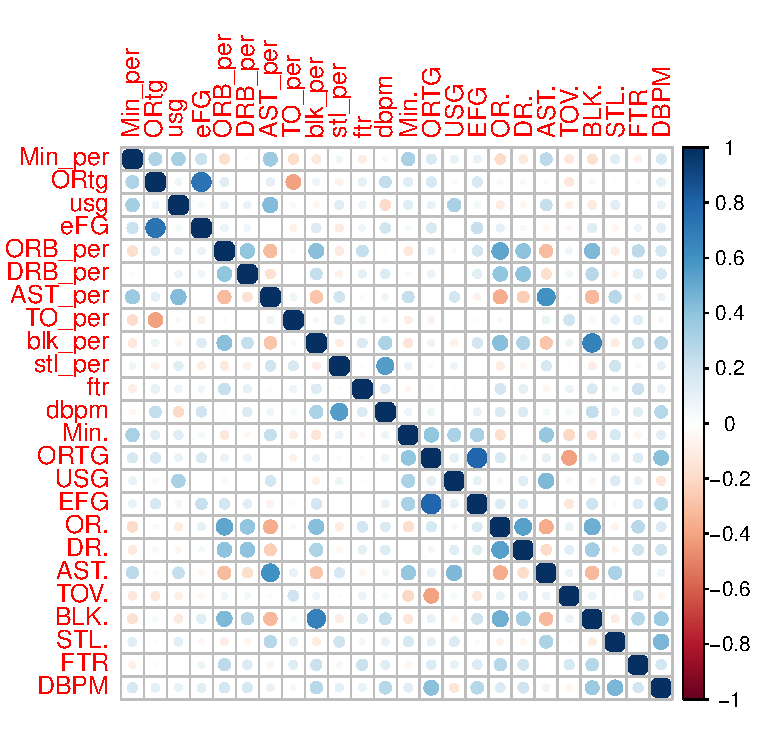
\includegraphics[width=\textwidth]{corrplot}
	\caption{A correlation matrix plot of the variables in the dataset.}
	\label{fig:corrplot}
\end{figure}

\subsection{Offensive Model}
\label{subsec:olm}
In the linear model to predict the next season's offensive efficiency, the statistically significant factors at the .05 significance level were ORtg, ORB\_per, AST\_per, ftr, fromp5, Min_per, and usg. \autoref{fig:olm.test.error} shows the absolute errors on the test set of the model. There are many outliers in this model due to players having very high or low metrics due to playing very little the year before they transferred. The root mean squared error on the test set of this model is 12.53. The model does perform well when predicting whether or not players will improve or not the next year in offensive rating. The model predicted 77.2\% of the players who improved their offensive rating correctly, and 67.4\% of the players who did not improve their offensive rating correctly, for an overall correct prediction rate of 73.2\%. When the model is re-run, but this time only with significant factors from the first running of the model, the root mean squared test error is lowered to 12.27. This time, the model correctly predicts 74.0\% of improvements and 70.6\% of non-improvements, for an overall correct rate of 72.6\%. The results of these two models are also shown in \autoref{tab:olm-results}. While the model's MAE is a bit high, it appears to do well when predicting improvements and non-improvements for players. In section~\ref{sec:cms}, we will see if setting the model's goal as classifying improvements and non-improvements helps these metrics.

\begin{figure}[tbp]
	\centering
	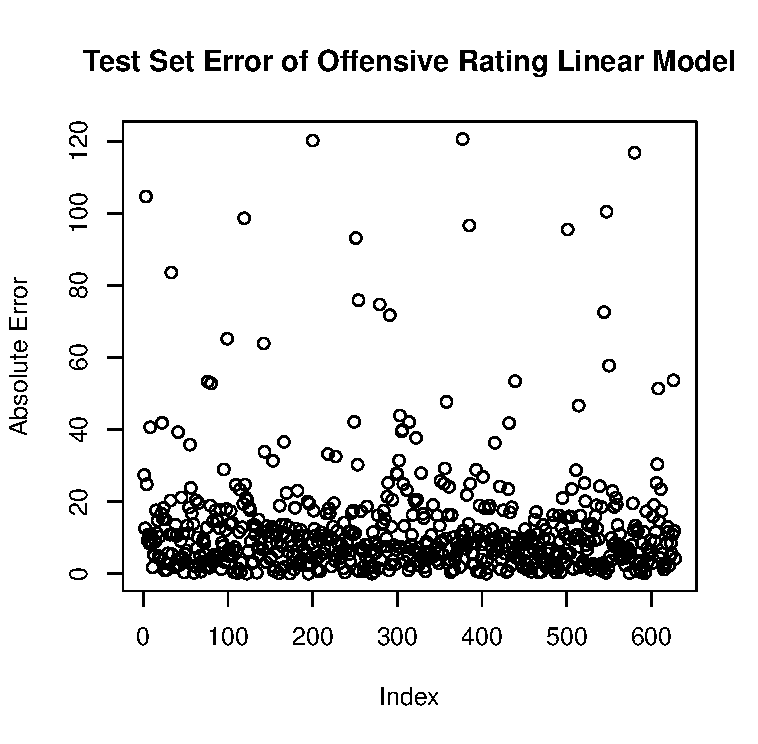
\includegraphics[width=\textwidth]{olm.test.error}
	\caption{A plot of the absolute test set error from the offensive linear model.}
	\label{fig:olm.test.error}
\end{figure}

\begin{table*}[t]
\centering
\resizebox{\textwidth}{!}{
\begin{tabular}{ccccc}
\toprule
Model & MAE & Correct Improvement & Correct Non-improvement & Overall Correct \\
\midrule
First Linear Model & 12.53 & 77.2\% & 67.4\% & 73.2\% \\
Significant Predictors Only & 12.27 & 74.0\% & 70.6\% & 72.6\% \\
\bottomrule
\end{tabular}
}
\caption{Offensive Linear Model Evaluators}
\label{tab:olm-results}
\end{table*}


\subsection{Defensive Model}
\label{subsec:dlm}
In the linear model to predict the following season's defensive box plus minus, the statistically significant factors at the .05 significance level were dbpm, DRB\_per, blk\_per, fromp5, top5, and Min\_per. \autoref{fig:dlm.test.error} shows the absolute errors on the test set for this model. Similarly to the offensive model, there are some outliers due to players having very little playing time. The MAE on the test set of this model is 1.22. Since dbpm is read on a different scale than ORtg, we cannot compare the MAE's of the models to determine which is easier to predict, although I will compare the MAE's of different types of models for offense and defense. In terms of predicting improvement, this model correctly predicted 75.6\% and 72.7\% of improvements and non-improvements, respectively. The overall correct prediction rate for this model is 74.2\%. Defensive improvement is a bit more inconsistent than offensive improvement, as it is less of a certainty for a player to improve their defensive traits year over year than their offensive ones. This means in theory, predicting defensive improvement is a bit more difficult, but this model actually predicts it at a similar rate as the offensive model did. When the model is re-run to only include significant factors, the MAE on the test set remains 1.22. The classification rates of this model are 76.3\% for improvements and 73.1\% for non-improvements, for an overall rate of 74.7\%. The summary of these results is also shown in \autoref{tab:dlm-results}.


\begin{figure}[tbp]
	\centering
	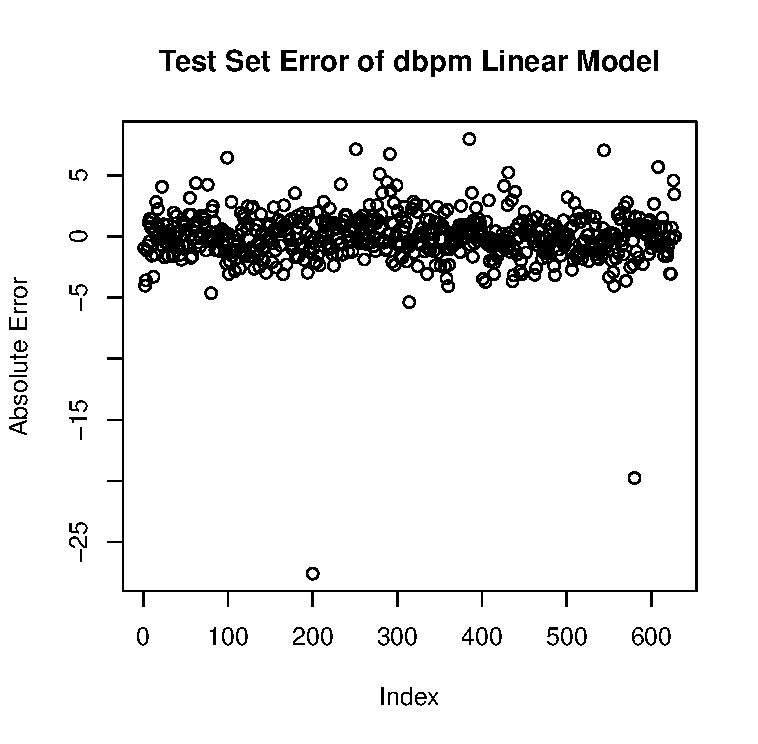
\includegraphics[width=\textwidth]{dlm.test.error}
	\caption{A plot of the absolute test set error from the defensive linear model.}
	\label{fig:dlm.test.error}
\end{figure}

\begin{table*}[t]
\centering
\resizebox{\textwidth}{!}{
\begin{tabular}{ccccc}
\toprule
Model & MAE & Correct Improvement & Correct Non-improvement & Overall Correct \\
\midrule
First Linear Model & 1.22 & 75.6\% & 72.7\% & 74.2\% \\
Significant Predictors Only & 1.22 & 76.3\% & 73.1\% & 74.7\% \\
\bottomrule
\end{tabular}
}
\caption{Defensive Linear Model Evaluators}
\label{tab:dlm-results}
\end{table*}


\section{Classification Models}
\label{sec:cms}
Since the linear models performed better when attempting to classify improvements and non-improvements, I next moved on to creating a model based solely on classifying these two outcomes. A similar style using logistic regression was followed for each model as in \autoref{sec:lms}, where offensive and defensive improvement were examined separately. Again, 70\% of the data was used for a training the model and the other 30\% was used for testing. While the MAE does not technically exist for logistic models, there is a very similar metric known as the Brier Score, which is given by 
\begin{equation}
  BS=\frac{1}{N}\sum_{i=1}^{N}(x_{i}-p_{i})^{2}.
\end{equation}
I used this metric on the test set in place of MAE for the classification models. While the Brier Score will not be on the same scale as the MAE of the linear models since it is comparing probability differences, we do now have the ability to compare the offensive and defensive models on the same scale.

\subsection{Offensive Model}
\label{subsec:ocm}
The statistically significant factors in the logistic model trying to predict offensive improvement were ORtg, TO\_per, fromp5, Min\per, and usg. When compared to the significant factors from the  linear model, ORB\_per and AST\_per are no longer significant, while TO\_per becomes significant. The Brier Score of this model is 0.19. The model correctly predicted 80.7\% of improvements, yet it only correctly predicted 60.0\% of non-improvements. The overall successful prediction rate of this model was 72.1\%, so even though the improvement and non-improvement percentages fluctuated, the overall correct percentage remained about the same as in the linear models. When only significant factors are used in the model, the Brier Score slightly increases to 0.19. The successful improvement prediction rate becomes 78.8\%, and the successful non-improvement prediction rate becomes 63.1\%. The overall correct prediction rate of this model is increased to 72.3\%. Finally, when the model is re-run with the same factors used in the final linear regression model, which were ORtg, ORB\_per, AST\_per, ftr, fromp5, Min_per, and usg, the Brier Score is 0.19. This model is able to successfully predict 80.7\% of improvements and 61.2\% of non-improvements. Overall, the correct prediction rate for this model is 72.6\%. The results of these models are summarized in \autoref{tab:ocm-results}.

\begin{table*}[t]
\centering
\resizebox{\textwidth}{!}{
\begin{tabular}{ccccc}
\toprule
Model & Brier Score & Correct Improvement & Correct Non-improvement & Overall Correct \\
\midrule
First Classification Model & 0.19 & 80.7\% & 60.0\% & 72.1\% \\
Significant Predictors Only & 0.19 & 78.8\% & 63.1\% & 72.3\% \\
Same Predictors as Significant in Linear Model & 0.19 & 80.7\% & 61.2\% & 72.6\% \\
\bottomrule
\end{tabular}
}
\caption{Offensive Classification Model Evaluators}
\label{tab:ocm-results}
\end{table*}


\subsection{Defensive Model}
\label{subsec:dcm}
In the logistic model to predict defensive improvement, dbpm, DRB\_per, blk\_per, stl\_per, fromp5, top5, and Min\_per are significant. In comparison to the linear defensive model, the only change is that stl\_per is now significant. All of the defensive predictors used are statistically significant in this model, so the model only using significant predictors is the same as the model using all the predictors. The Brier Score of this model is 0.18, which is slightly better than any of the offensive classification models. The model correctly predicted 76.6\% of improvements in dbpm and 71.1\% of non-improvements. Overall, this model correctly predicted 73.9\% of the improvements and non-improvements correctly, which is again slightly better than the offensive classification models. When we modify the model to include the same parameters that were found significant in the linear defensive model, the Brier Score remains 0.18. Now, the model correctly predicts 79.1\% of defensive improvements. The non-improvement prediction rate lowered to 68.8\%, and the overall successful prediction rate increased slightly to 74.0\%. These results are also summarized in \autoref{tab:dcm-results}.

\begin{table*}[t]
\centering
\resizebox{\textwidth}{!}{
\begin{tabular}{ccccc}
\toprule
Model & Brier Score & Correct Improvement & Correct Non-improvement & Overall Correct \\
\midrule
First Classification Model & 0.18 & 76.6\% & 71.1\% & 73.9\% \\
Significant Predictors Only & 0.18 & 76.6\% & 71.1\% & 73.9\% \\
Same Predictors as Significant in Linear Model & 0.18 & 79.1\% & 68.8\% & 74.0\% \\
\bottomrule
\end{tabular}
}
\caption{Offensive Classification Model Evaluators}
\label{tab:dcm-results}
\end{table*}

\section{Machine Learning Numerical Prediction Models}
\label{sec:mlnp}
Next, I moved on to attempting to predict transfer success using machine learning techniques, specifically neural networks. The same training and testing split was used as in the linear and logistic models. For both offensive and defensive models, one hidden layer, a batch size of 50, the ReLU activation function, and an epoch length of 300 were used to fit the model. RMSprop, which is an improved version of gradient descent, was used as the optimizer when compiling the model. More information about the RMSprop optimizer can be found here. (CITE KERAS LINK) The layer sizes of the neural networks varied a bit due to the different number of predictors used in the offensive and defensive models. CITE PAPER HERE proposes that the best number of neurons to use in a one hidden layer neural network is \(n = N + 1\), where N is equal to the number of inputs. With an output layer of one neuron, it is then suggested that N neurons are used in the hidden layer, which is the strategy I chose to follow. For both models, the loss function used is MSE. The same metrics as used for the linear regression models were used for the machine learning models.

\subsection{Offensive Model}
\label{subsec:omlnp}
For the offensive model, all predictors were used. These predictors were ORtg, eFG, ORB\_per, AST\_per, TO\_per, ftr, fromp5, top5, Min\_per, and usg. Following the strategy outlined in \autoref{sec:mlnp}, 11 neurons were used in the hidden layer of the model. \autoref{fig:omlnp.test.error} shows the absolute error on the test set of the model. The model has an MAE of 9.93 on the test set. This model was excellent in terms of classification. It successfully predicted 97.6\% of improvements as well as 97.6\% of non-improvements, for an overall rate of 97.6\%. So, while the MAE, is comparable to the linear offensive model, this model does a much better job of classifying players. These results are summarized in \autoref{tab:omlnp-results}.

\begin{figure}[tbp]
	\centering
	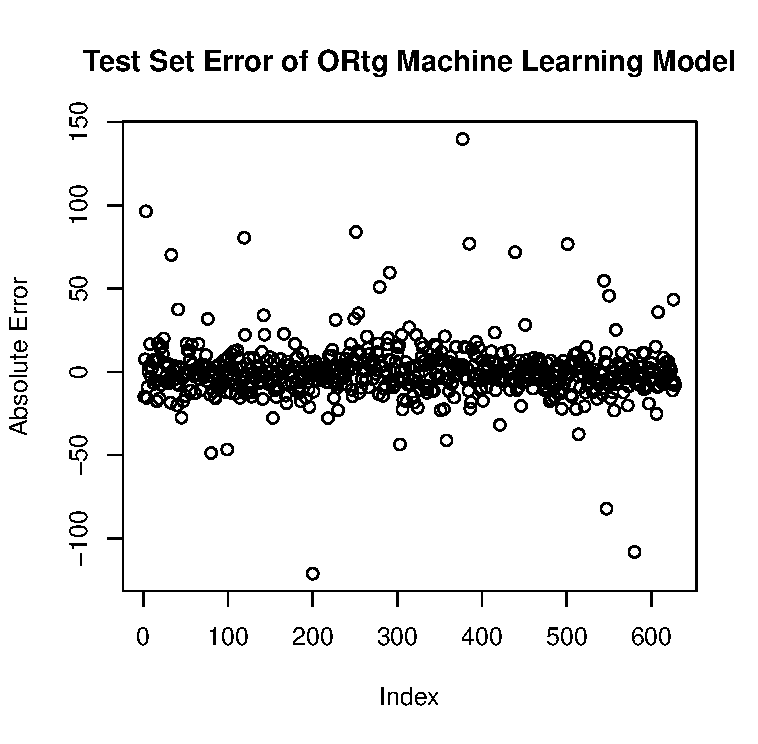
\includegraphics[width=\textwidth]{omlnp.test.error}
	\caption{A plot of the absolute test set error from the offensive machine learning model.}
	\label{fig:omlnp.test.error}
\end{figure}

\begin{table*}[t]
\centering
\resizebox{\textwidth}{!}{
\begin{tabular}{ccccc}
\toprule
Model & MAE & Correct Improvement & Correct Non-improvement & Overall Correct \\
\midrule
Neural Network Model & 9.93 & 97.6\% & 97.6\% & 97.6\% \\
\bottomrule
\end{tabular}
}
\caption{Offensive Neural Network Model Evaluators}
\label{tab:omlnp-results}
\end{table*}

\subsection{Defensive Model}
\label{subsec:dmlnp}
Similar to the offensive model, all available predictors were used. These predictors were dbpm, DRB\_per, blk\_per, stl\_per, Min\_per, fromp5, and top5. Again, following the same strategy outlined in \autoref{sec:mlnp}, 7 neurons were used in the hidden layer. The absolute error on the test set is shown in \autoref{fig:dmlnp.test.error}. This model performed  closely to the previous defensive model. It had a MAE of 1.34. It successfully predicted 76.9\% of improvements and 70.1\% of non-improvements for an overall correct prediction rate of 73.6\%.  The results are summarized in \autoref{tab:dmlnp-results}.

\begin{figure}[tbp]
	\centering
	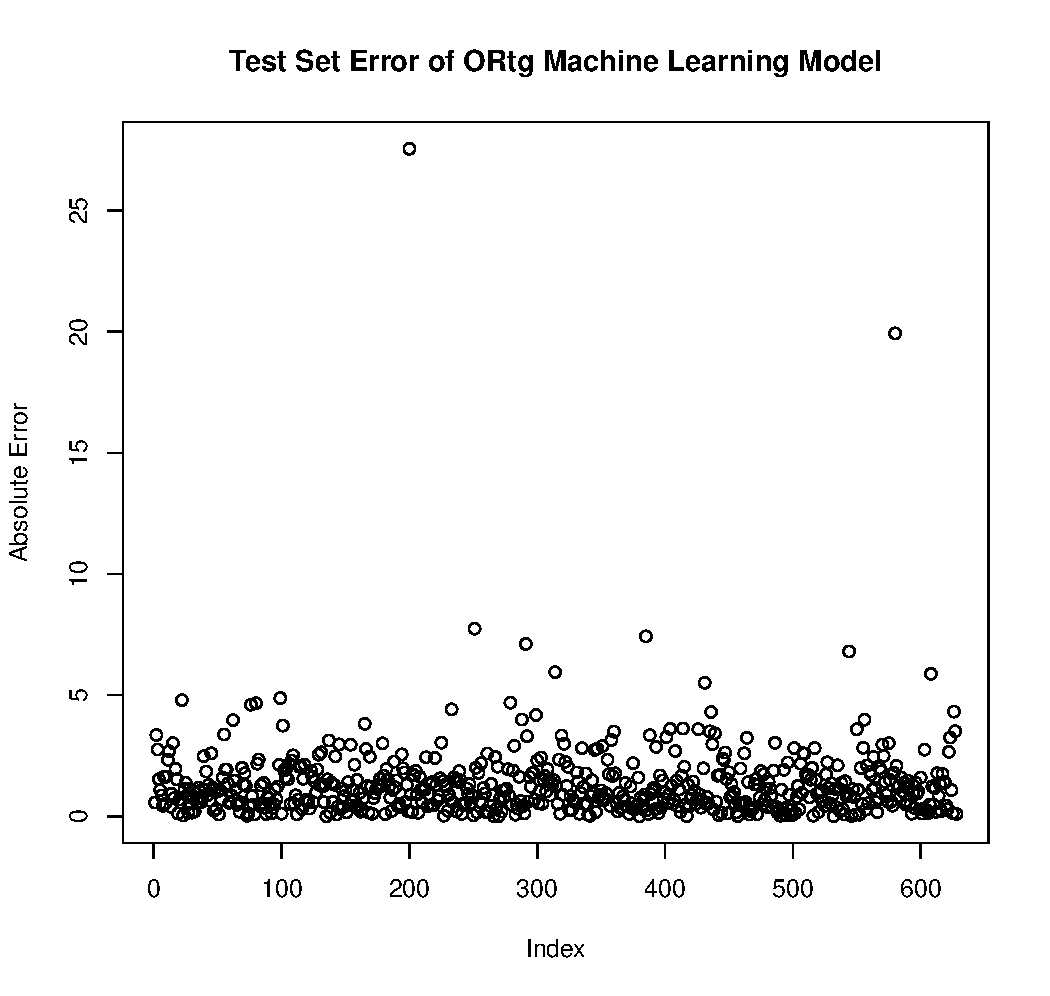
\includegraphics[width=\textwidth]{dmlnp.test.error}
	\caption{A plot of the absolute test set error from the defensive machine learning model.}
	\label{fig:dmlnp.test.error}
\end{figure}

\begin{table*}[t]
\centering
\resizebox{\textwidth}{!}{
\begin{tabular}{ccccc}
\toprule
Model & MAE & Correct Improvement & Correct Non-improvement & Overall Correct \\
\midrule
Neural Network Model & 1.34 & 76.9\% & 70.1\% & 73.6\% \\
\bottomrule
\end{tabular}
}
\caption{Defensive Neural Network Model Evaluators}
\label{tab:dmlnp-results}
\end{table*}

\section{Machine Learning Classification Models}
\label{sec:mlc}
The process of building a classification neural network is very similar to one for numerical prediction, with a few changes. Since the output layer will have two neurons because we are doing binary classification, these models will have \(n=N+2\) neurons. I made the choice to change to this strategy in order to keep the number of neurons in the hidden layer consistent so we can more easily compare models. In this case, for the output layer, the sigmoid (or logistic) activation function is used. The loss function used in this case is binary cross entropy, which is considered the best loss function to use for classification tasks. For consistency, the same batch size and epoch length are used for these models. Brier Score is once again used to evaluate these classification models

\subsection{Offensive Model}
\label{subsec:omlc}
For this offensive model, again all predictors were used. These predictors were ORtg, eFG, ORB\_per, AST\_per, TO\_per, ftr, fromp5, top5, Min\_per, and usg. 11 neurons were once again used in the hidden layer. This model had a Brier Score of 0.36. It correctly predicted 80.7\% of offensive improvements and 61.2\% of defensive improvements. The overall successful prediction rate the model was 72.6\%. The results are summarized in \autoref{tab:omlc-results}.

\begin{table*}[t]
\centering
\resizebox{\textwidth}{!}{
\begin{tabular}{ccccc}
\toprule
Model & Brier Score & Correct Improvement & Correct Non-improvement & Overall Correct \\
\midrule
Neural Network Classification Model & 0.36 & 80.7\% & 61.2\% & 72.6\% \\
\bottomrule
\end{tabular}
}
\caption{Offensive Neural Network Classification Model Evaluators}
\label{tab:omlc-results}
\end{table*}

\subsection{Defensive Model}
\label{subsec:dmlc}
For the defensive model, all predictors were once again used. These predictors were dbpm, DRB\_per, blk\_per, stl\_per, Min\_per, fromp5, and top5. I used 7 neurons in the hidden layer. This model's Brier Score was 0.35. It predicted 78.1\% of defensive improvements and 69.5\% of defensive non-improvements. The overall correct prediction rate was 73.9\%. The results of this model are summarized in \autoref{tab:dmlc-results}. 

\begin{table*}[t]
\centering
\resizebox{\textwidth}{!}{
\begin{tabular}{ccccc}
\toprule
Model & Brier Score & Correct Improvement & Correct Non-improvement & Overall Correct \\
\midrule
Neural Network Classification Model & 0.35 & 78.1\% & 69.5\% & 73.9\% \\
\bottomrule
\end{tabular}
}
\caption{Defensive Neural Network Classification Model Evaluators}
\label{tab:dmlc-results}
\end{table*}


\end{document}